\documentclass[11pt]{exam}

\usepackage{amssymb, amsmath, amsthm, mathrsfs, multicol, graphicx}
\usepackage{tikz, pgfplots}


\def\d{\displaystyle}
\def\?{\reflectbox{?}}
\def\b#1{\mathbf{#1}}
\def\f#1{\mathfrak #1}
\def\c#1{\mathcal #1}
\def\s#1{\mathscr #1}
\def\r#1{\mathrm{#1}}
\def\N{\mathbb N}
\def\Z{\mathbb Z}
\def\Q{\mathbb Q}
\def\R{\mathbb R}
\def\C{\mathbb C}
\def\F{\mathbb F}
\def\A{\mathbb A}
\def\X{\mathbb X}
\def\E{\mathbb E}
\def\O{\mathbb O}
\def\pow{\mathscr P}
\def\inv{^{-1}}
\def\nrml{\triangleleft}
\def\st{:}
\def\~{\widetilde}
\def\rem{\mathcal R}
\def\iff{\leftrightarrow}
\def\Iff{\Leftrightarrow}
\def\and{\wedge}
\def\And{\bigwedge}
\def\AAnd{\d\bigwedge\mkern-18 mu\bigwedge}
\def\Vee{\bigvee}
\def\VVee{\d\Vee\mkern-18 mu\Vee}
\def\imp{\rightarrow}
\def\Imp{\Rightarrow}
\def\Fi{\Leftarrow}


\def\bar{\overline}

%\pointname{pts}
\pointsinmargin
\marginpointname{pts}
\marginbonuspointname{ bns pts}

\addpoints
\pagestyle{headandfoot}
%\printanswers


\header{MATH 131}{\bf\large Learning Target 19 Quiz}{Fall 2025}
\runningfooter{}{}{Version \version}
\extrafootheight{-.45 in}



\begin{document}
\def\version{A}
%space for name
\noindent {\large\bf Name:} \underline{\hspace{2.5 in}}
\vskip 1em

\begin{questions}
\question Consider the function $f(x)$ graphed below.

\begin{center}
    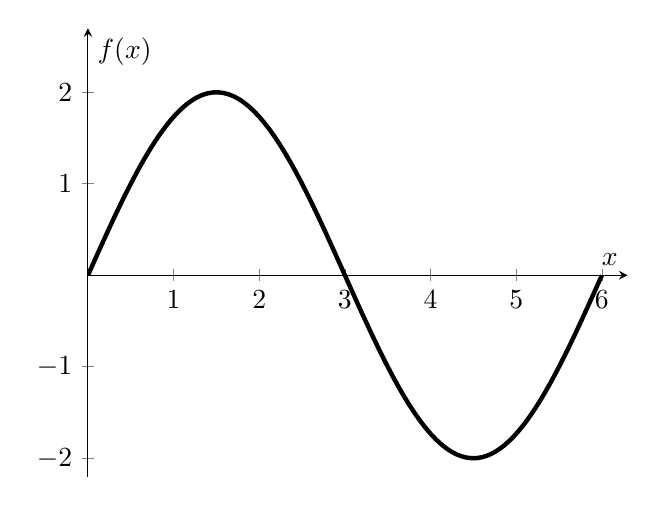
\begin{tikzpicture}[
      declare function={
        func(\x) = {2*sin(deg(1/3*pi*\x))};
      }
    ]
      \begin{axis}[
        axis x line=middle, axis y line=middle, ymin=-2.2, ymax=2.7, xmin=0, xmax=6.3, xlabel=$x$, ylabel=$f(x)$, grid=none
      ]
        \addplot [domain=0:6, samples=100, ultra thick]{func(x)};
      \end{axis}
    \end{tikzpicture}
\end{center}
\begin{parts}
\part Give the exact value of $\int_0^6 f(x)\, dx$.  Briefly explain your answer.
\vfill
\part Write an expression in terms of one or more integrals, that gives the total area between the curve and the $x$-axis.
\vfill
\end{parts}
\end{questions}

\newpage

\def\version{B}
%space for name
\noindent {\large\bf Name:} \underline{\hspace{2.5 in}}
\vskip 1em


\begin{questions}
\question Consider the function $f(x)$ graphed below.  Assume each portion of the graph is either part of a line or part of a circle.

\begin{center}
    \begin{tikzpicture}[
      declare function={
        func(\x) = (\x <= 2)*(sqrt(1-(\x-1)^2)) + and(\x > 2, \x <=4) * (abs(\x - 3)-1);
      }
    ]
      \begin{axis}[
        axis x line=middle, axis y line=middle, ymin=-1.5, ymax=1.9, xmin=0, xmax=4.3, xlabel=$x$, ylabel=$f(x)$, grid=none
      ]
        \addplot [domain=0:4, samples=100, ultra thick]{func(x)};
      \end{axis}
    \end{tikzpicture}
\end{center}
\begin{parts}
\part Give the exact value of $\int_0^4 f(x)\, dx$.  Briefly explain your answer.
\vfill
\part Write an expression in terms of one or more integrals, that gives the total area between the curve and the $x$-axis.
\vfill
\end{parts}
\end{questions}

\newpage

\def\version{C}
%space for name
\noindent {\large\bf Name:} \underline{\hspace{2.5 in}}
\vskip 1em

\begin{questions}
\question Consider the function $f(x)$ graphed below. Assume each portion of the graph is either part of a line or part of a circle.

\begin{center}
    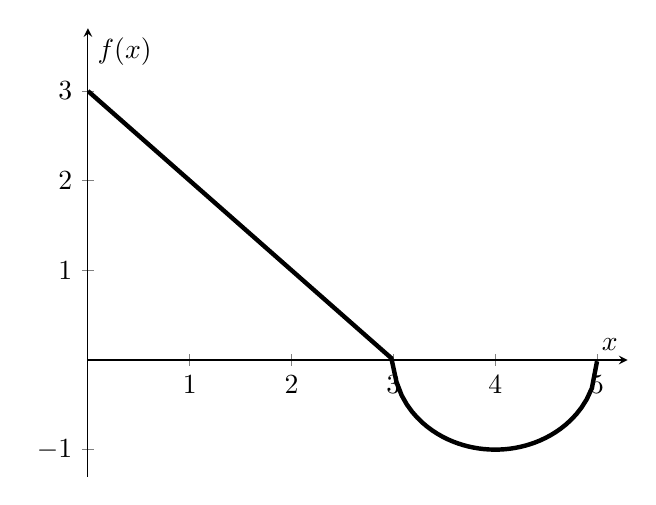
\begin{tikzpicture}[
      declare function={
        func(\x) = (\x <= 3)*(3-\x) + (\x > 3)*(-sqrt(1-(\x-4)^2));
      }
    ]
      \begin{axis}[
        axis x line=middle, axis y line=middle, ymin=-1.3, ymax=3.7, xmin=0, xmax=5.3, xlabel=$x$, ylabel=$f(x)$, grid=none
      ]
        \addplot [domain=0:5, samples=100, ultra thick]{func(x)};
      \end{axis}
    \end{tikzpicture}
\end{center}
\begin{parts}
\part Give the exact value of $\int_0^5 f(x)\, dx$.  Briefly explain your answer.
\vfill
\part Write an expression in terms of one or more integrals, that gives the total area between the curve and the $x$-axis between $x=0$ and $x = 5$.
\vfill
\end{parts}
\end{questions}

\newpage

\def\version{D}
%space for name
\noindent {\large\bf Name:} \underline{\hspace{2.5 in}}
\vskip 1em

\begin{questions}
\question Consider the function $f(x)$ graphed below.  Assume each portion of the graph is either part of a line or part of a circle.

\begin{center}
    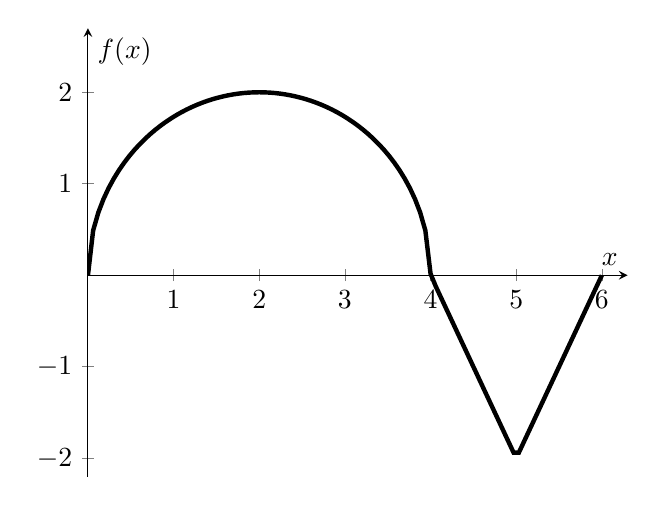
\begin{tikzpicture}[
      declare function={
        func(\x) = (\x <= 4)*(sqrt(4-(\x-2)^2)) + and(\x > 4, \x <= 6) * (2*abs(\x - 5)-2);
      }
    ]
      \begin{axis}[
        axis x line=middle, axis y line=middle, ymin=-2.2, ymax=2.7, xmin=0, xmax=6.3, xlabel=$x$, ylabel=$f(x)$, grid=none
      ]
        \addplot [domain=0:6, samples=100, ultra thick]{func(x)};
      \end{axis}
    \end{tikzpicture}
\end{center}
\begin{parts}
\part Give the exact value of $\int_0^6 f(x)\, dx$.  Briefly explain your answer.
\vfill
\part Write an expression in terms of one or more integrals, that gives the total area between the curve and the $x$-axis.
\vfill
\end{parts}
\end{questions}

\end{document}
